\section{Proof Maintenance}
\label{sec:mot-mai}

What does it mean to \textit{maintain} a verified system?
Like all software systems, verified systems evolve over time.
The difference is that, for verified systems, the proofs must evolve alongside the rest of the system (Section~\ref{sec:changes}).
Proof engineers typically use development processes to make proofs less likely to break in the 
face of these changes (Section~\ref{sec:design-robust}).
Still, even with good development processes, breaking changes happen all the time, even for experts (Section~\ref{sec:irl}).
All of this points to a need for change-aware proof automation---that is, proof repair.

\subsection{Breaking Changes}
\label{sec:changes}

At its core, a verified system has three parts, corresponding to the workflow from Section~\ref{sec:mot-dev}:

\begin{enumerate}
\item programs,
\item specifications, and
\item proofs.
\end{enumerate}
As verified systems evolve over time, both programs and specifications can change.
Either of these changes can break existing proofs.

Consider the example from Section~\ref{sec:verif}.
We had two choices for the specification of \lstinline{zip_preserves_length}.
We chose the weaker specification on the left of Figure~\ref{fig:zip-pres}.
This gives us some freedom in how we implement our \lstinline{zip} function.
At some point, we may wish to change \lstinline{zip}, and update our proof so that it still holds.
Alternatively, we may wish to port our development to use the stronger specification on the right of Figure~\ref{fig:zip-pres}
We may even wish to use a datatype more expressive than \lstinline{list}, as we will see in Section~\ref{TODO}. % TODO
Any of these changes can break proofs in our proof development.

\paragraph{Changing our Program}

Our specification of \lstinline{zip_preserves_length} gives us some freedom to change how our \lstinline{zip} function from Figure~\ref{fig:zip} behaves on edge cases,
when the lengths of input lists are not equal.
Suppose we change our \lstinline{zip} function to always return \lstinline{nil} in those cases,
by just returning the old behavior when the lengths are equal, and otherwise returning \lstinline{nil}.
To do this, we rename our old \lstinline{zip} function to be \lstinline{zip_same_length}.
We then define a new \lstinline{zip} function that breaks into those two cases, calling \lstinline{zip_same_length}
when the lengths are equal, and otherwise returning \lstinline{nil}:

\begin{lstlisting}
zip {T$_1$} {T$_2$} (l$_1$ : list T$_1$) (l$_2$ : list T$_2$) : list (T$_1$ * T$_2$) :=
  sumbool_rect (fun _ => list (T$_1$ * T$_2$))
    (fun (_ : length l$_1$ = length l$_2$) =>
      zip_same_length l$_1$ l$_2$)
    (fun (_ : length l$_1$ <> length l$_2$) =>
      nil)
    (eq_dec (length l$_1$) (length l$_2$)).
\end{lstlisting}
where \lstinline{sumbool_rect} is an eliminator that lets us break into these two cases, and 
\lstinline{eq_dec} says that equality is decidable over natural numbers (that is, any two numbers are either equal or not equal).

% TODO we want this to work with PUMPKIN PATCH original, but will need some programming time for that to actually happen...

Our theorem \lstinline{zip_preserves_length} still holds, but after changing our program, the \textit{proof} that it holds breaks.
We can fix it by adding the \codediff{highlighted} tactics:

\begin{lstlisting}
Proof.
  (@\codediff{intros. unfold zip.}@)
  (@\codediff{induction (eq\_dec (length l$_1$) (length l$_2$)); try contradiction.}@)
  (@\codediff{simpl. revert a. revert H. revert l$_2$.}@)
  induction l$_1$ as [|t$_1$ tl$_1$ IHtl$_1$].
  - auto.
  - intros l$_2$. induction l$_2$ as [|t$_2$ tl$_2$ IHtl$_2$].
    + intros H. auto.
    + intros H. simpl. rewrite IHtl1; auto.
Defined.
\end{lstlisting}
If we have many proofs about \lstinline{zip}, they may break in similar ways, and require similar patchwork.

\paragraph{Changing our Specification}
Suppose we had instead chosen the stronger specficiation on the right of Figure~\ref{fig:zip-pres},
and kept our \lstinline{zip} function the same.
We can update our proof accordingly, but after changing this specification, other proofs may break.
For example, if we had written a lemma for the \lstinline{cons} case:

\begin{lstlisting}
Lemma zip_preserves_length_cons :
  $\forall$ {T$_1$ : Type} {T$_2$ : Type} (l$_1$ : list T$_1$) (l$_2$ : list T$_2$) (t$_1$ : T$_1$) (t$_2$ : T$_2$),
    length l$_1$ = length l$_2$ $\rightarrow$
    length (zip (cons t$_1$ l$_1$) (cons t$_2$ l$_2$)) = S (length l$_1$).
Proof.
  intros T$_1$ T$_2$ l$_1$ l$_2$ t$_1$ t$_2$ H.
  simpl. f_equal.
  rewrite zip_preserves_length; auto.
Defined.
\end{lstlisting}
that followed by \lstinline{zip_preserves_length},
then after the change, this proof would break.

We would have two choices to fix it. Either we could leave our specification alone,
and fix our proof.
In that case,
the proof would look like this instead (with the difference \codediff{highlighted}):

\begin{lstlisting}
Proof.
  intros T$_1$ T$_2$ l$_1$ l$_2$ t$_1$ t$_2$ H.
  simpl. f_equal.
  (@\codediff{rewrite $\leftarrow$ min\_id. rewrite H at 2.}@)
  apply zip_preserves_length; auto.
Defined.
\end{lstlisting}
The extra tactics correspond to an extra proof obligation:
we must now show that \lstinline{length l}$_1$\lstinline{ = min (length l}$_1$\lstinline{) (length l}$_2$\lstinline{)}.
This holds by the lemma \lstinline{min_id} from the Coq standard library, combined with the hypothesis that says that \lstinline{length l}$_1$\lstinline{= length l}$_2$.

Alternatively, we could strengthen the specification of that lemma as well, and leave the proof alone:

\begin{lstlisting}
Lemma zip_preserves_length_cons :
  $\forall$ {T$_1$ : Type} {T$_2$ : Type} (l$_1$ : list T$_1$) (l$_2$ : list T$_2$) (t$_1$ : T$_1$) (t$_2$ : T$_2$),
    length (zip (cons t$_1$ l$_1$) (cons t$_2$ l$_2$)) = S (min (length l$_1$) (length l$_2$)).
Proof.
  intros T$_1$ T$_2$ l$_1$ l$_2$ t$_1$ t$_2$.
  simpl. f_equal.
  apply zip_preserves_length_alt; auto.
Defined.
\end{lstlisting}
But this could continue to break other downstream proofs that depend on \lstinline{zip_preserves_length_cons},
causing a cascading effect of change.

\subsection{Designing Robust Proofs}
\label{sec:design-robust}

Proof engineers often use development processes to work around some of the challenges of change to begin with (Section~\ref{sec:design}).
For example, they might use information hiding techniques~\cite{Woos:2016:PCF:2854065.2854081, Klein:2014:CFV:2584468.2560537}
to abstract away the details of \lstinline{zip} or of \lstinline{zip_preserves_length},
so that the burden of change becomes just showing that the changed program or proof still implements that abstraction.
Similarly, they may build their own custom tactics that hide the details of
\lstinline{zip} or \lstinline{zip_preserves_length} behind the automation itself,
so that the burden of change becomes just fixing the automation.

But design principles like this all rely on proof engineers having the right foresight to choose the 
right abstractions in the right places, and hide the right information behind them.
And it turns out that proof enginers do not always have perfect foresight.
They may write proofs that depend on details like the names of variables or the names of lemmas,
much like our proofs in Section~\ref{sec:changes}.
Or they may choose abstractions to hide information, but those may not be the abstractions they still want after the change,
or they may hide the wrong information behind the abstractions.
Worse, breaking changes may happen outside of the proof engineers' control,
in libraries upon which their proof developments depend.

All of this is why, even with good development processes, even expert proof engineers
sometimes still struggle with change.
In other words, even experts are human.

\subsection{Even Experts are Human}
\label{sec:irl}

% TODO include REPLICA diagram and so on

Even with good development processes, proof engineers change programs and specifications all the time---and this does break proofs, 
even for experts.
To find evidence of this in the real world, \kl{Alex} and I built a Coq plugin called \toolname 
(REPL Instrumentation for Coq Analysis) that listens to the Read Eval Print
Loop (REPL)---a simple loop that all user interaction with Coq passes through---to collect data that the proof engineer sends to Coq during development.
%This includes data difficult to obtain from other sources, like failed
%proof attempts and incremental changes to definitions.
We used \toolname to collect a month's worth of granular data on 
the proof developments of 8 intermediate to expert Coq users.
We visualized and analyzed this data to classify hundreds changes to programs and specifications,
and fixes to broken proofs.
The resulting data, analyses, and proof repair benchmarks are publicly available with the proof engineers' 
consent.\footnote{\url{http://github.com/uwplse/analytics-data}}

\begin{figure}
  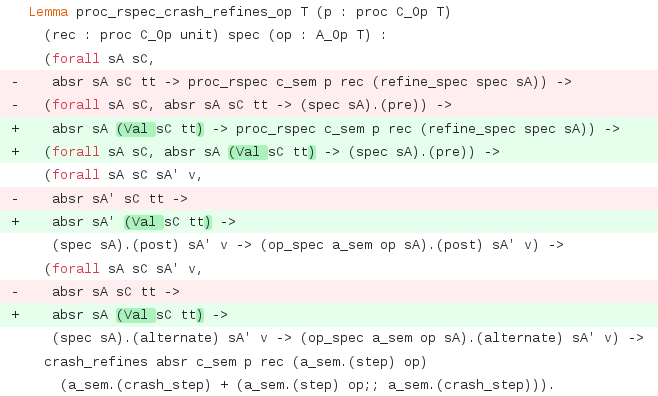
\includegraphics[width=1.0\textwidth]{maintenance/fig/patch.png}
  \caption{Patches to a lemma by an expert proof engineer.}
  \label{fig:patch}
\end{figure}

We found that changes to programs and specifications were often formulaic and repetitive.
For example, Figure~\ref{fig:patch} shows an example change by an expert proof engineer.
In this change, the proof engineer wraps two arguments into a single application of \lstinline{Val}
in three different hypotheses of a lemma.
This change did not occur in isolation: the proof engineer patched 10 other definitions or lemmas
in similarly, wrapping arguments into an application of
\lstinline{Val}.
%I suspect that this was due to a change in the definition of \lstinline{absr},
%but I was not able to confirm this since
%the change in question occurred before the beginning of the study.

We also found that changes to programs and specifications did break proofs, even for expert proof engineers.
The proof engineers most often (75\% of the time) fixed broken proofs by stepping 
up above those proofs in the UI and fixing something else, like a specification.
That is, development and maintenance were in reality tightly coupled.

But sometimes, proof engineers did not successfully fix proofs broken by changes in programs and specifications.
For example, for the change in Figure~\ref{fig:patch},
the expert proof engineer admitted or aborted (that is, gave up on) the proofs of four of the five
broken lemmas after this change.
In other words, right now, even experts sometimes just give up in the face of change.

% TODO left off here

(The rest of this subsection is not done yet, but not really needed to understand flow.)
And it's an extra big problem when you have a large development and the changes are outside of your control.

Hence Social Processes.

Why automation breaks, even with good development processes.
In other words, even experts are human.
And automation doesn't understand how things change, so can't help the human out.
But proof repair---smarter proof automation---can.

% TODO for now, just a copy-paste of analytics original paper, including the bib---will change soon

%\section{Introduction}

%Proof assistants allow programmers to verify everything from distributed systems~\cite{wilcox:verdi} and compilers~\cite{leroy:compcert} to
%formalizations of mathematics~\cite{DBLP:journals/corr/BauerGLSSS16}. 

Proof automation makes verification more accessible to programmers, but it is often intractable
without programmer guidance. In \textit{interactive theorem proving} (ITP), the programmer guides the 
proof search process. The guidance reduces the search space to make proof automation more tractable.
This in turns helps the programmer, who does not have to manually verify the entire system.

%Interactive theorem provers allow programmers to guide proof search and interactively 
%verify everything from distributed systems~\cite{wilcox:verdi} and compilers~\cite{leroy:compcert} to
%formalizations of mathematics~\cite{DBLP:journals/corr/BauerGLSSS16}. In many of these theorem provers, programmers use

%In these languages, programmers write precise specifications of programs
%and prove implementations correct with respect to the specifications.

Despite automation, programming in these proof assistants is brittle: Even a minor change to a definition or theorem
can break many dependent proofs. This is a major source of development inefficiency in proof assistants
based on dependent type theory~\cite{proof-eng, Aydemir2008, Delaware2013ICFP}.

Traditional proof automation does not consider how proofs, definitions, and theorems change over time.
Instead, it is driven by the state of the current proof, sometimes with supplementary
information from other proofs, definitions, and theorems (as in hint databases~\cite{hints} and rippling~\cite{rippling}).
This puts the burden of dealing with brittleness on the programmer. 

We present a new approach to proof automation that accounts for breaking changes. %:
%searching the difference in versions of a proof, definition, or theorem. 
%We reimagine the problem of proof reuse~\cite{Boite2004, Mulhern06proofweaving} 
%in the context of traditional automation for ITP. 
In our approach, the programmer guides proof search 
by providing an \textit{example} of how to adapt proofs to changes in definitions or theorems.
A tool then generalizes the example adaptation into a \textit{reusable patch} that the programmer can use to fix
other broken proofs.

In doing so, we chart a path for a future %of ITP 
that moves the burden of brittleness
away from the programmer and into proof automation. 
Programmers typically address brittleness through design principles that make proofs
resilient to change~\cite{proof-eng, Aydemir2008, Delaware2013ICFP}, or through program-specific proof automation~\cite{chlipala:cpdt}.
These techniques, while useful, have limitations: 
Planning a verification effort around future change is challenging, and program-specific automation requires specialized knowledge.
The programmer's ability to anticipate likely changes determines the robustness of both techniques in
the face of change. %The robustness of both techniques in the face of change is determined by the programmer's ability to anticipate likely changes. 
Even then, many breaking changes are outside of the programmer's control. Updating proof assistant
versions, for example, can break proofs regardless of planning or automation~\cite{verdicommit}.

\begin{figure*}[ht]
\begin{minipage}{0.48\textwidth}
\centering
\lstset{language=coq, aboveskip=0pt, belowskip=0pt}
\lstinputlisting[firstline=1, lastline=3]{repair/izr.tex}
\lstinputlisting[backgroundcolor=\color{orange!35},firstline=4,lastline=5]{repair/izr.tex}
\lstinputlisting[firstline=6, lastline=6]{repair/izr.tex}
\end{minipage}
\hfill
\begin{minipage}{0.48\textwidth}
\centering
\lstset{language=coq, aboveskip=0pt, belowskip=0pt}
\lstinputlisting[firstline=8, lastline=10]{repair/izr.tex}
\lstinputlisting[backgroundcolor=\color{orange!35},firstline=11,lastline=12]{repair/izr.tex}
\lstinputlisting[firstline=13, lastline=13]{repair/izr.tex}
\end{minipage}
\vspace{-.3cm}
%\setlength{\belowcaptionskip}{-2pt}
\caption[Caption]{Old (left) and new (right) definitions of \lstinline{IZR} in Coq.
The old definition applies injection from naturals to reals and conversion of positives to
naturals; the new definition applies injection from positives to reals.}
\label{fig:izr}
\end{figure*}


We identify a set of core components that are critical to searching an example for patches in Coq.
We use the components to build %four different 
a procedure for finding patches %for non-structural changes 
in a Coq plugin as a 
proof-of-concept.
Case studies on real projects like CompCert~\cite{leroy:compcert} and the Coq standard library
suggest that patches are useful for realistic scenarios, and that it is simple to compose the components 
to handle different classes of changes.
We test the boundaries of the components on a suite of tests
and show how our findings can help build the future we envision.

In summary, we contribute the following:

\begin{enumerate}
%\item We develop new foundations for proof automation in ITP that account for breaking changes. % TODO reword
\item We identify a set of core components that are key to searching for patches.
\item We demonstrate that these core components are useful on real changes in Coq code.
\item We explore how to drive a future that moves the burden of change in ITP away from the programmer and into automated tooling.
\end{enumerate}

% TODO fix contributions

% evaluation stuff in contributions too

% SOMEWHERE: we focus on non-structural changes





%\section{Building \toolname}
\label{sec:plugin}

\toolname is a tool that collects fine-grained proof development data.
%without relying on a particular UI.
It is available on Github for Coq 8.10, with backported branches for
Coq 8.8 and Coq 8.9.\footnote{\url{http://github.com/uwplse/coq-change-analytics}}

\toolname works by instrumenting Coq to listen to user interaction.
Coq's interaction model (Section~\ref{sec:repl}) implements a REPL,
or Read Eval Print Loop: a loop that continually reads in messages
from the user, evaluates the statements those messages contain, 
and prints responses to the user.
All UIs for Coq, from the command line tool
\lstinline{coqtop}~\cite{coq-commands} to the IDEs CoqIDE~\cite{coqide} and
Proof General~\cite{Aspinall2000}, communicate with Coq through the REPL.
\toolname instruments the REPL to collect fine-grained data while remaining
decoupled from the UI.

Figure~\ref{fig:design} summarizes the design of \toolname.
\toolname is made of two parts: a client that the user installs,
and a web server that stores the data from multiple users.
The client instruments the REPL to record and log the data that the
user's UI sends to Coq (Section~\ref{sec:client}),
then sends this data to the server (Section~\ref{sec:server}),
which stores it for analysis.

The implementation effort for \toolname was modest, with just 412 LOC
of OCaml for the client and 178 LOC of Python for the server.%
\footnote{Counted using David M. Wheeler's SLOCCount.}
This modest effort was enough for us to collect 
(Section~\ref{sec:deployment}) and analyze 
(Sections~\ref{sec:q1} and~\ref{sec:q2}) data from hundreds
of interactive sessions.

\subsection{User-Coq Interaction}
\label{sec:repl}

% Is there a better source than this: http://paral-itp.lri.fr/papers/files/coq-workshop-paper.pdf
The \toolname client listens for messages that the user's UI
sends to Coq's REPL.
To provide a common API for different UIs, the implementation of
Coq's REPL is organized into an interactive state machine.
Each state can include tactics in Coq's tactic language Ltac or commands
in Coq's vernacular; both of these can reference terms in Coq's
specification language Gallina.
When a UI sends a message to Coq's REPL, the message contains a state
machine statement (a labeled transition) that instructs Coq to do one of three things:

\begin{enumerate}
\item \textit{Add}: produce a new state
\item \textit{Exec}: execute an existing state to receive a response
\item \textit{Cancel}: back up to an existing state
\end{enumerate}
Coq reacts accordingly, then returns an ID for the new state
that corresponds to the statement.

Taken together, these three statement types can be used
to reconstruct the proof engineer's behavior,
such as defining and redefining types, interactively constructing proofs,
and stepping up when the user hits a dead-end.

% Talia: Trying to get latex to display this in a reasonable place
\begin{figure}
  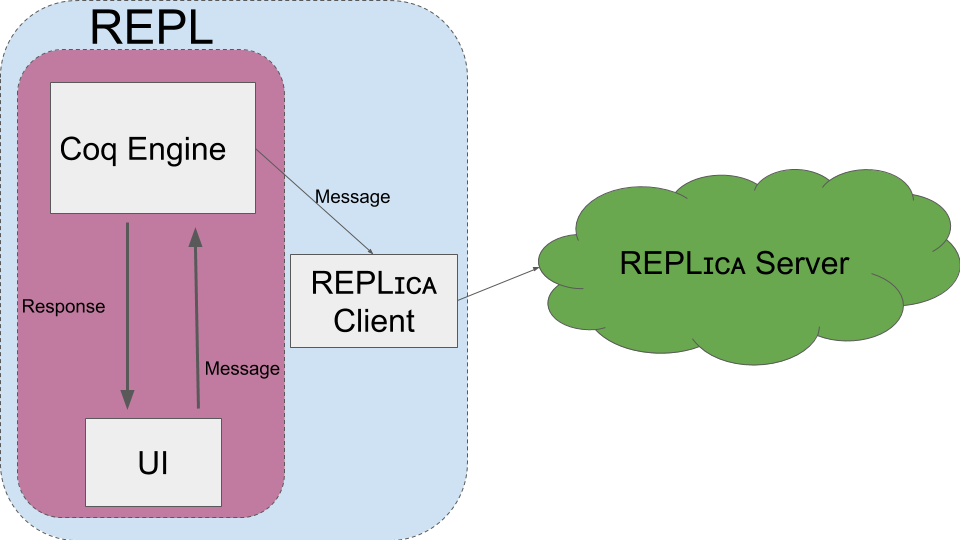
\includegraphics[width=0.8\columnwidth]{maintenance/fig/architecture.png}
\caption{\toolname design. The \toolname client listens to the REPL
and sends data to the \toolname server.}
\label{fig:design}
\end{figure}

\paragraph{From User Behavior to the State Machine}
When the user runs a command or tactic in Coq, the UI first adds
a new state corresponding to the command or tactic.
Adding a state to the state machine does not actually execute the
command or tactic;
to do that, the UI must execute the new state.
In other words, in state machine terms, each addition follows a transition,
but only returns the state number.
To get the state information, the UI must call \textit{Exec}.

Using this mechanism, the UI can group state machine statements and execute them
all at once. %, without interacting with the intermediate states.
For example, stepping down past 3 definitions at once in an IDE
manifests as 3 additions followed by a constant
number of executions, and successfully compiling a file manifests as 
many additions followed by a constant number of 
executions.\footnote{Some UIs send Coq multiple executions for each
group of additions.} 

When the user steps up in the UI, or attempts to run a tactic or command
that fails, the UI backs up to an existing state in the state machine.
Sending the state machine a cancellation statement is not the only way to back up to
an existing state; cancellations can also take the form of state machine
\textit{additions} of \lstinline{Cancel} or \lstinline{BackTo} commands
in Coq's vernacular. In either form, cancellations take a state ID
as an argument to specify the state to back up to.
%% Trying a statement that fails manifests as a cancellation,
%% and stepping up in an IDE manifests as a cancellation
%% followed by an IDE signature;
%% Section~\ref{sec:discussion} discusses distinguishing between these.

\paragraph{An Example: Defining and Extending an Inductive Type}
To see how user behavior corresponds to state machine statements,
consider an example from User 1, Session 41, simplified for readability.
In this session, User 1 stepped past
the definition of an inductive type \lstinline{Alpha}. Later, User 1
stepped above \lstinline{Alpha}, imported list notations,
then stepped down to add a new constructor to \lstinline{Alpha}
using those notations.

When User 1 first stepped down below \lstinline{Alpha},
Coq received a state machine addition (denoted
\lstinline{Add}, following SerAPI~\cite{GallegoArias2016SerAPI})
of this definition (again simplified for readability):

\begin{lstlisting}
  (Add () "Inductive Alpha : $\ldots$ := $\ldots$")
\end{lstlisting}
at the state ID \lstinline{1}, producing state ID \lstinline{2}.
Since User 1 stepped down a single step, Coq also received
an execution (denoted \lstinline{Exec}) of the new state:

\begin{lstlisting}
  (Exec 2)
\end{lstlisting}
which did not produce a state with a new state ID, since only additions
produce states, and only states have state IDs.
When User 1 stepped up to above the definition of \lstinline{Alpha},
Coq received a cancellation (denoted \lstinline{Cancel}):

\begin{lstlisting}
  (Cancel 1)
\end{lstlisting}
taking the state machine to before the definition of \lstinline{Alpha}.
When User 1 added the import, Coq
received an addition at state ID \lstinline{1}, producing state ID
\lstinline{3}, followed by an execution:

\begin{lstlisting}
  (Add () "Import Coq.Lists.List.ListNotations. ")
  (Exec 3)
\end{lstlisting}
Finally, when User 1 added the new constructor to \lstinline{Alpha}
and stepped down past it,
Coq received an addition of \lstinline{Alpha} with the new
constructor at state ID  \lstinline{3} producing state ID \lstinline{4}, followed by an execution:

\begin{lstlisting}
  (Add () "Inductive Alpha : $\ldots$ := $\ldots$
             | alpha_rec_mt : $\ldots$")
  (Exec 4)
\end{lstlisting}

The data that \toolname received provided us with enough
information to visualize these changes as a sequence of
diffs for later analysis (Section~\ref{sec:q2}).
As a consequence, we were able to find this pattern of development
of incrementally extending inductive types for four of our users
(Section~\ref{sec:pat1}).

\subsection{User-Client Interaction}
\label{sec:client}

The \toolname client records all of the additions, executions,
and cancellations that the proof engineer's UI or compiler sends.
To use it, the proof engineer installs the client,
then adds a line to the Coq requirements file~\cite{coqrc} so that
Coq always loads it.
On the first build, \toolname asks the proof engineer for consent and
for demographic information for the study.
From then on, the proof engineer uses Coq normally.

The implementation of the client is a Coq plugin.
Coq's plugin system makes it possible to extend
Coq without compromising trust in the Coq core.
\toolname does not include new commands or tactics; it simply attaches
to Coq's REPL and listens for messages that the proof engineer sends to Coq.

The hooks in the plugin API that allow plugins to listen to the REPL
were not initially present in Coq;
we worked with one of the Coq developers
to add this to Coq 8.10.\footnote{\url{http://github.com/coq/coq/pull/8768}}
We also developed backported branches of Coq 8.8 and 8.9 that include
this API, so that users whose projects depended on those
versions of Coq could participate in our study. This API is now available in all
versions of Coq going forward. %so that other study and plugin authors
%can use it.

\subsection{Client-Server Interaction}
\label{sec:server}

To record a history of user behavior,
the \toolname client sends a record of each state machine addition,
execution, and cancellation to the \toolname server.
The server then collects this data into a format suitable for analysis.

The message that the client sends to the server includes both the
state machine statement and additional metadata.
\iffalse
For example, a full message to the server for the simplified example
from Section~\ref{sec:repl} looks like this:

\begin{lstlisting}
((time 1567665712.25)
 (id 2)
 (user 1)
 (session-module gamma_completeness_implies_ec_assoc)
 (session 1567665710.63)
 (Control
   (Add () "Inductive Alpha : $\ldots$ := $\ldots$")))
\end{lstlisting}
where \lstinline{time} is the time the state change occurred,
\lstinline{id} is the state of the addition,
\lstinline{user} is the user ID,
\lstinline{session-module} is the Coq module in which the statements
were executed,
\lstinline{session} is the start time of the session,
and the body of the messages beginning with \lstinline{Control}
is the addition to the state machine.
%\todo{what do we do about our off-by-one errors?}
\fi

\begin{figure*} % Talia: For good table placement
\begin{minipage}{0.67\textwidth}
\small
\centering
\begin{tabular}{ |l|l|l|l|l|l|l| }
 \hline
  \textbf{User} & \textbf{Years} & \textbf{Expertise} & \textbf{Purpose} & \textbf{Frequency} & \textbf{UI} & \textbf{Version} \\
\hline
  \textbf{0} & 2-4 & $\circ$ $\circ$ $\circ$ $\circ$ $\circ$ & Verification & Daily & Proof General & Master \\
  \textbf{1} & 2-4 & $\circ$ $\circ$ $\circ$ & Mathematics & Monthly & Proof General & 8.10 \\
  \textbf{2} & > 4 & $\circ$ $\circ$ $\circ$ $\circ$ & Verification & Daily & Proof General & 8.10 \\
  \textbf{3} & > 4 & $\circ$ $\circ$ $\circ$ $\circ$ $\circ$ & Verification & Weekly & Proof General & Master \\
  \textbf{4} & > 4 & $\circ$ $\circ$ $\circ$ $\circ$ & Verification & Daily & coqtop & Master \\
  \textbf{5} & 2-4 & $\circ$ $\circ$ $\circ$ & Verification & Monthly & Custom & 8.10 \\
  \textbf{6} & 2-4 & $\circ$ $\circ$ $\circ$ $\circ$ & Mathematics & Daily & Proof General & Master \\
  \textbf{7} & 2-4 & $\circ$ $\circ$ $\circ$ $\circ$ & Mathematics & Weekly & Proof General & 8.10 \\
  \textbf{8} & > 4 & $\circ$ $\circ$ $\circ$ $\circ$ $\circ$ & Verification & Daily & Proof General & 8.8 \\
  \textbf{9} & > 4 & $\circ$ $\circ$ $\circ$ $\circ$ $\circ$ & Verification & Monthly & Proof General & 8.9 \\
  \textbf{10} & > 4 & $\circ$ $\circ$ $\circ$ & Verification & Daily & Proof General & 8.8 \\
  \textbf{11} & > 4 & $\circ$ $\circ$ $\circ$ & Mathematics & Daily & Proof General & 8.9 \\
\hline
\end{tabular}
\caption{User profiles of Coq development
background: experience in years, self-assessed expertise (beginner, novice, intermediate, knowledgeable, or expert, represented by circles), purpose of use, frequency of use, UI, and current version.}
\label{tab:users}
\end{minipage}
\hfill
\begin{minipage}{0.31\textwidth}
\small
\centering
\begin{tabular}{ |l|l|l|l| }
 \hline
  \textbf{User} & \textbf{Total} & \textbf{Interactive} & \textbf{Proof}\\
\hline
  \textbf{0} & 6 &  0 & 0 \\
  \textbf{1} & 42 & 10 & 4 \\
  \textbf{2} & 7 & 3 & 0 \\
  \textbf{3} & 11495 & 101 & 8 \\
  \textbf{4} & 1 & 0 & 0 \\
  \textbf{5} & 41 & 15 & 16 \\
  \textbf{6} & 1 & 0 & 0 \\
  \textbf{7} & 229 & 183 & 241 \\
  \textbf{8} & 162 & 27 & 10 \\
  \textbf{9} & 5 & 0 & 0 \\
  \textbf{10} & 23 & 15 & 0 \\
  \textbf{11} & 17 & 8 & 0 \\
\hline
\end{tabular}
\caption{Number of total sessions, interactive sessions,
  and interactive proof subsessions per user.}
\label{tab:sessions}
\end{minipage}
\end{figure*}

\paragraph{Metadata for Two Challenges}
The metadata beyond the state ID and the state machine
statement exists to handle two challenges:
The first challenge is that state machine interactions alone
are not enough to reconstruct a per-user history,
nor to group the user's interaction into discrete sessions
for a particular project or module.
The second challenge is that the network can be slow or unreliable at times,
causing messages to be received by the server out of order,
and slowing down the UI if not handled properly.

To handle the first challenge, \toolname labels each message with
a module name, user ID, and session ID.
The module name comes from the Coq plugin API.
The user ID is generated by the server and stored on the user's machine.
\iffalse
When a user builds the client for the first time, it contacts the server
and receives a unique user ID, which is stored locally on the
user's machine.
\fi
The session ID, in contrast, is generated by the client:
When the user loads the client, upon opening any new file,
the client records the start time of the session.
This start time is then used to identify the session.

To handle the second challenge, \toolname{} labels each message
with two pieces of metadata: the time at which the state machine message was sent to Coq (to order messages)
and the state ID (to detect missing states).
TCP alone is not enough to address these issues since each invocation
of the plugin creates a separate network stream
(so the server may receive messages out of order),
and since the user can disable the plugin
(so the client may never send some 
messages).\footnote{The consent form allowed users to temporarily disable
the plugin if necessary, as long as they informed us of this.} 
In addition to this metadata,
%instead of sending messages as soon as they are ready,
\toolname{} sends messages in batches.
If the network is not available, \toolname{} logs messages locally,
then sends those logs to the server the next time
the network is available.


%\section{Deploying \toolname}
\label{sec:deployment}

We set out to answer the following questions:

\begin{itemize}
\item \textbf{Q1}: What kinds of mistakes do users make in interactive proofs, and how do they fix them? (Section~\ref{sec:q1})
\item \textbf{Q2}: What kinds of changes to programs and specifications do users
make often, and do those changes reveal patterns amenable to automation? (Section~\ref{sec:q2})
\end{itemize}
To answer these questions, we recruited 12 proof
engineers to install \toolname and use Coq normally for
a month (Section~\ref{sec:recruiting}).
We received a month's worth of data containing granular detail on
Coq development for 8 of 12 of those users
(Section~\ref{sec:collection}).
After a month, we shut down the server, closed the study,
and visualized and analyzed the data (Section~\ref{sec:analysis}).

\subsection{Recruiting}
\label{sec:recruiting}

We recruited proof engineers by distributing a promotional video
and study description.
\iffalse
 to the \lstinline{coq-club} email list, on Twitter,
and directly to professors at universities with many Coq users.
\fi
All potential users went through a screening process, ensuring that they are
at least 18 years old, fluent in English, and have at least a year of experience using Coq.
Upon installation of the plugin, users filled out a consent form.
Users then filled out a questionnaire about Coq background and usage,
the results of which are in Figure~\ref{tab:users}.

All users reported more than 2 years of experience;
7 reported more than 4.
Self-assessed expertise was evenly distributed between intermediate,
knowledgeable, and expert; no beginners or novices participated.
4 users reported that they use Coq for writing mathematical proofs,
while the other 8 reported that they use Coq for verifying software.
7 users said that they use Coq every day, 2 a few times per week,
and 3 a few times per month.
10 users reported using Proof General, while 1 user reported using
\lstinline{coqtop}, and 1 user reported using a custom UI.
4 users installed the plugin with the master branch of Coq,
while 4 users used Coq 8.10, 2 users used Coq 8.9,
and 2 users used Coq 8.8.

\subsection{Collection}
\label{sec:collection}

The study period lasted one month, during which users agreed to develop
Coq code with the plugin enabled whenever possible, or otherwise let us know
why this was not possible.
All of the data collected within this time period
has been made publicly available with the consent of the users.\footnote{\url{http://github.com/uwplse/analytics-data}}

Figure~\ref{tab:sessions} shows the number of sessions by user.
Every time the plugin was loaded, either inside of a compiled file
or inside of a file open in a UI, this began a new session.
For both Q1 and Q2, our analyses looked for changes only within
sessions that involved some combination of failure
and stepping up and then back down in a UI;
we call these \textit{interactive sessions}.

We marked a session as interactive if it contained at least
one cancellation followed by other changes in
state. This did not capture any compilation passes
because Coq disallows cancellations outside of interactive mode.
For example, User 3 logged 11495 total sessions, only 101
of which were interactive. 
The remainder of User 3's sessions were, for the most part,
compilation passes over large sets of dependencies (one session per dependency).
In total, across all users, there were 362 interactive sessions.

Within these interactive sessions, the analysis for Q1 looked for 
fixes to failing tactics only inside of spans of time spent 
\emph{inside proofs} that involved some combination of failure and
stepping up and then back down in a UI;
we call these \textit{interactive proof subsessions}.
There could be zero, one, or multiple of these within an interactive session.
We detected these similarly to how we detected
interactive sessions.
There were 279 interactive proof subsessions.

\toolname logged interactive sessions for only 8 of the 12 users.
Section~\ref{sec:discussion} discusses possible causes of, implications of,
and remedies for this.
%We speculate as to why, consider the implications,
%and discuss how to reach more users in Section~\ref{sec:discussion}.

\subsection{Analysis}
\label{sec:analysis}

Once we had collected this data, we analyzed it to answer Q1 and Q2.
To answer these questions, we developed a small Python
codebase to analyze the data.
The scripts used information about cancellations
to build visualizations to aid in analysis.
For Q1, we built this cancellation information into a search tree for
each proof, and produced visualizations of each tree
(see \Cref{fig:search-tree}).
For Q2, we used this cancellation
information to reconstruct a sequence of diffs, and used Git tooling
to manually inspect these diffs (see \Cref{fig:ex-diff}).

The scripts, visualizations, and results for Q1 and Q2 can
be found alongside the data in the public data repository. 

\section{Q1: Mistakes In and Fixes to Proofs}
\label{sec:q1}

Q1 asked what mistakes proof engineers
make in proofs, and how they fix those mistakes.
This data may inform the development of tools
that help users write proofs
by suggesting next steps and changes to existing tactics.

\paragraph{A1}
We found the following:

\begin{enumerate}
\item Most interactive proof subsessions ended
  in the user stepping up to an earlier definition.
This shows that writing definitions and proofs about those definitions was
usually a feedback loop. (Section~\ref{sec:feedback})
\item Within proofs, application of lemmas
was the main driver of proving. (Section~\ref{sec:tactics})
\item Within proofs, over half of fixes to tactic mistakes
fixed either an improper argument or wrong sequencing structure.
(Section~\ref{sec:fixes})
\end{enumerate}

\paragraph{Methodology}
Our analysis for Q1 looked within the 279 interactive proof subsessions.
We first counted the number of times each tactic was used, the number
of times it was stepped above, and the number of times its invocation
caused an error. Then, we constructed a search tree using the
cancellation structure, and for any state which had multiple out edges
(a proof state where multiple tactics were tried), we compared the
cancelled attempts to the final tactic used.

\subsection{Fixing Proofs by Fixing Definitions}
\label{sec:feedback}

Of the 279 interactive proof subsessions, 209 (over 75\%) began a proof,
only to step above the entire proof attempt and
return to make changes to earlier definitions or commands, for example
to change a specification to make the proof possible.
This suggests that tools that attempt to provide next steps to users writing proof
may also benefit from suggesting possible fixes to definitions used in the proof.
% ,as the proof often cannot be completed without first changing definitions.
% ^ Talia: We can't claim "often cannot," but I think it's OK to omit
\begin{displayquote}
  \textbf{Takeaway:}
  It may be beneficial to combine machine learning tools
  that automatically complete or suggest hints for
  proofs~\cite{proverbot9001, Komendantskaya2012, Nagashima2018, Gauthier2017b,
    Yang2019}
  with tools for repairing definitions~\cite{Ringer2018, robert2018}.
\end{displayquote}

We considered only the remaining 70 successful interactive proof subsessions
(made up of 1085 tactic invocations)
for the sake of analyzing behavior \textit{within} proofs that
ended in a successful proof.
The analysis for Q2 (Section~\ref{sec:q2}) reveals more about
how specifications and programs changed.

\begin{figure}
\small
  \begin{tabular}{|l|c|c|c|}
    \hline
    \textbf{Tactic} & \textbf{Used} & \textbf{Failed} & \textbf{Stepped Above} \\
    \hline
    apply& 156& 27& 13\\
    intros& 108& 16& 5\\
    destruct& 94& 24& 12\\
    rewrite& 61& 13& 12\\
    exists& 47& 9& 1\\
    unfold& 45& 2& 8\\
    simpl& 32& 6& 4\\
    reflexivity& 27& 1& 1\\
    simpl in& 25& 3& 7\\
    assumption& 24& 2& 1\\
    specialize& 19& 0& 1\\
    subst& 14& 1& 0\\
    split& 12& 0& 0\\
    eapply& 11& 0& 5\\
    dependent& 10& 0& 8\\
    inversion& 10& 0& 0\\
    constructor& 10& 3& 0\\
    eauto& 9& 0& 4\\
    assert& 9& 2& 0\\
    induction& 8& 0& 1\\
    validate& 8& 0& 5\\
    monoid& 7& 0& 2\\
    tauto& 7& 1& 0\\
    eassumption& 7& 0& 5\\
    repeat constructor& 7& 0& 5\\
    \hline
  \end{tabular}
  \caption{The top 25 most common tactics.}
\label{fig:tactics-table}
\end{figure}

\subsection{Tactics Used and Cancelled}
\label{sec:tactics}

\begin{figure*}
  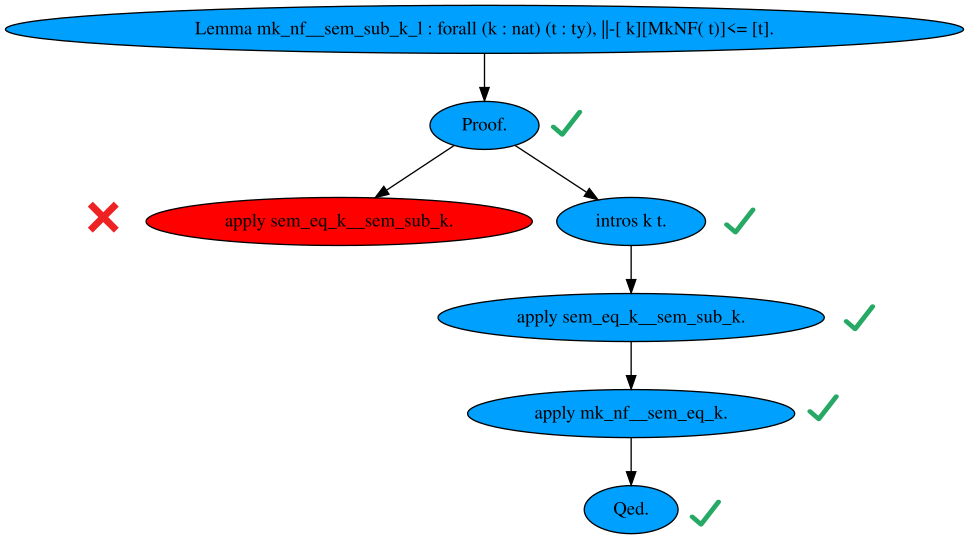
\includegraphics[width=0.70\textwidth]{maintenance/fig/example-graph.png}
  \caption{An example search tree, generated from the collected data
    by \toolname. It shows the user attempting to apply a lemma, which
    fails until they first run the \lstinline{intros} tactic.}
  \label{fig:search-tree}
\end{figure*}

\Cref{fig:tactics-table} shows the counts for each tactic
(regardless of arguments) in the 70 successful interactive proof subsessions.
%From this table, we can see that the
The distribution of tactics run was top-heavy; over 50\% of the tactics
invoked were either \lstinline{apply}, \lstinline{intros},
\lstinline{destruct}, \lstinline{rewrite}, \lstinline{exists}, \
\lstinline{unfold}, or \lstinline{simpl}.
The \lstinline{apply} tactic had a significant lead over other tactics
in invocations, but invocations of \lstinline{destruct} ended in
failure or stepping above them nearly as many times as invocations
of \lstinline{apply} did.

This data indicates two takeaways for proof tooling:
Firstly,
\begin{displayquote}
  \textbf{Takeaway:}
  Tools may be able to focus on understanding the behavior of
  and suggesting just a small number of tactics,
  and still benefit.
\end{displayquote}
And second, since lemma and hypothesis application was the main driver of proofs,
\begin{displayquote}
  \textbf{Takeaway:}
  Assessing which lemmas and hypotheses are useful would be one of the main tasks of
  a tool which suggests tactics to the user.
\end{displayquote}
The machine learning tool ML4PG~\cite{Komendantskaya2012} for Coq
already offers promising developments in this direction by understanding
and providing hints about similar lemmas,
as does the proof automation tool CoqHammer~\cite{coqhammer};
similar functionality may help
improve the performance of tools that suggest tactics.

\subsection{Fixing Proofs by Fixing Tactics}
\label{sec:fixes}

%While the raw cancellation numbers are useful, they do not give a
The raw cancellation numbers do not give a
broader context to each cancellation, namely what tactic it was
cancelled in favor of. To address this, we built a search
graph and analyzed the tactic attempts at each branching node (see
\Cref{fig:search-tree}). Where there were more than 2 attempts, we
compared all non-final attempts to the final one separately.

In our 71 successful interactive proof subsessions, 96 tactics
were cancelled in favor of another tactic at the same state.
Of the 96 cancelled-tactic and final-tactic pairs: %, we found:
\begin{itemize}
\item 13 were semicolon clauses added after a tactic, like:
  \begin{lstlisting}
    destruct w. $\to$ destruct w; reflexivity.
  \end{lstlisting}
\item 4 were semicolon clauses removed from the end of a tactic, like:
  \begin{lstlisting}
    intros; reflexivity. $\to$ intros.
  \end{lstlisting}
\item 31 were the same tactic with modified arguments, like:
  \begin{lstlisting}
    intros k X t. $\to$ intros k X t Hfresh.
  \end{lstlisting}
\item 5 were similar, but a \lstinline{Search} or \lstinline{Check} command was first run
  before replacing the tactic, like:
  \begin{lstlisting}
    apply IdSetFacts.remove_3. $\to$ 
    Check IdSetFacts.remove_3. 
    apply IdSetFacts.remove_3 with Y.
  \end{lstlisting}
\item 43 changes did not fall into this categorization.
\end{itemize}

The proofs shown were complex, and users often made nontrivial
changes to attempted tactics, so not all changes could be
easily categorized or analyzed. However, over half of the changes
present could be categorized into simple changes, and potentially
synthesized by automated tools.

This data also shows us that for a large proportion of tactics, users
could correctly pick the tactic to invoke, even when they made
mistakes in its arguments. In addition, fixing these arguments took both
on average and in the worst case longer than fixing other kinds
of mistakes. Accordingly,
\begin{displayquote}
  \textbf{Takeaway:}
  Automated tooling that suggests actions to take
  based on tactics that were recently stepped above or failed
  may focus on predicting new arguments for the attempted tactic.
\end{displayquote}

\section{Q2: Changes to Terms}
\label{sec:q2}

Q2 asked what kinds of changes proof
engineers make to programs and specifications, and whether those
changes reveal patterns amenable to automation.
This information may be useful to ensure tools for proof evolution
support the features that help proof engineers.

\paragraph{A2}
We found that while no single change was dominant across
all users, users made related changes within and across sessions.
Analysis of these changes revealed four patterns:

\begin{enumerate}
\item Incremental development of inductive types
\item Repetitive refactoring of identifiers
\item Repetitive repair of specifications
\item Interactive discovery of programs and specifications
\end{enumerate}

\paragraph{Methodology}
To answer this question, we wrote a script to visualize changes over 
time as diffs on Github (see Figure~\ref{fig:ex-diff}).
The script reconstructed the state of the file up to 
each cancellation within a session, then committed that to the 
public data repository.
When possible (see Section~\ref{sec:wish2}), it augmented
each commit with information on whether the cancellation was a failure
or the user stepping up in an IDE.

We then manually analyzed the diffs that this visualization produced to 
build a classification of changes (Section~\ref{sec:class}), 
then classify changes that we found (Section~\ref{sec:changes}).
We did this for each of the 362 interactive sessions and, when relevant,
across sessions as well.
Finally, we looked at clusters of common changes for patterns.
For each of the four patterns we found
(Sections~\ref{sec:pat1},~\ref{sec:pat2},~\ref{sec:pat3}, and~\ref{sec:pat4}),
we identified benchmarks (examples of the pattern in our data)
and lessons for automation.

\subsection{Building a Classification}
\label{sec:class}

After running the visualization script, we did a manual analysis of the diffs
in order to build a classification of changes to Gallina terms.
This analysis was thorough in that it involved inspecting each
consecutive diff and, when relevant, diffs that spanned several commits
(when a user stepped up, changed something, and then later stepped back down)
or sessions (when a user modified the same file during two different sessions).
However, it did not necessarily capture all changes to terms;
Section~\ref{sec:wish2} discusses some of the challenges.

\paragraph{Classification}

We designed a classification that groups changes along three dimensions:

\begin{enumerate}
\item \textbf{Command}: vernacular command used to define the term in
                        which a subterm changed
\item \textbf{Operation}: how the subterm changed
\item \textbf{Location}: innermost subterm that changed
\end{enumerate}
with the following categories for \textbf{Operation}:

\begin{enumerate}
\item \textbf{Structure}:
\begin{enumerate}
\item \textbf{Add} or \textbf{Del}: add or delete information
\item \textbf{Mov}: move information
\end{enumerate}
\item \textbf{Content}:
\begin{enumerate}
\item \textbf{Pch} or \textbf{Uch}: patch or unpatch
\item \textbf{Cut} or \textbf{Uut}: cut or uncut
\item \textbf{Rpl}: replace
\end{enumerate}
\item \textbf{Syntax}:
\begin{enumerate}
\item \textbf{Rnm}: rename
\item \textbf{Qfy} or \textbf{Ufy}: qualify or unqualify
\end{enumerate}
\end{enumerate}
Changes listed together are inverse operations.
The \textbf{Structure} changes are straightforward.
Among the changes to \textbf{Content}, \textbf{Pch} is applying a function
to the old term to get a new term, \textbf{Cut} is defining a new term
or let-binding and then referring to that term inside of an existing term,
and \textbf{Rpl} is replacing contents in any other way.
Among the \textbf{Syntax} changes, \textbf{Qfy} is
qualifying a constant after changing an import.

For \textbf{Structure} changes, there are five \textbf{Location}s:

\begin{enumerate}
\item \textbf{Hyp}: hypothesis of anything that can take arguments
\item \textbf{Arg}: argument in an application
\item \textbf{Ctr}: constructor of an inductive type
\item \textbf{Cas}: case of a match statement
\item \textbf{Bod}: body of anything that can take arguments
\end{enumerate}

For \textbf{Content} changes, there are an additional two:

\begin{enumerate}
\setcounter{enumi}{5}
\item \textbf{Fun}: function in an application
\item \textbf{Typ}: type annotation
\end{enumerate}

For \textbf{Syntax} changes, there are only three:

\begin{enumerate}
\item \textbf{Bnd}: binding in the local environment
\item \textbf{Idn}: identifier in the global environment
\item \textbf{Con}: constant
\end{enumerate}

\paragraph{Design Considerations}

That classification that we designed considers changes only within
Gallina terms defined or stated using vernacular commands.
Since it is focused solely on changes to defined terms,
it does not consider other information like changes to vernacular commands,
hints, tactics, notations, scope annotations, inference information, or imports,
and it considers additions of new terms only in \textbf{Cut} changes.

In building this classification, we aimed to group
changes at a level of granularity narrow enough to inform the design of proof
engineering tools, but broad enough to capture patterns.
We suspect that within these categories, there are more granular
categories that can be useful for automation, like distinguishing among
hypotheses to set apart indices of inductive types, or classifying
a \textbf{Content} change as semantics-preserving.
We did not design a more granular classification because we did not
find it useful for describing our data.
%(we found no changes to indices of inductive types, for example).

\subsection{Classifying Changes}
\label{sec:changes}

Once we had designed this classification,
we used it to classify the changes that we had found.
We ignored intermediate changes that immediately failed to lex, parse, or type check.

\begin{figure*}
\small
\begin{tabular}{ |l|rrrr|l|l|l| }
\hline
     \textbf{User} &
     \multicolumn{4}{c|}{\textbf{Top Changes}} &
     \textbf{\# Changes} &
     \textbf{\# Interactive} &
     \textbf{Expertise}
\\
\hline
     \textbf{1} &
     \indpat{\textbf{Add} \textbf{Ctr} (23)} &
     \indpat{\textbf{Add} \textbf{Cas} (22)} &
     \refactorpat{\textbf{Qfy} \textbf{Con} \phantom{0}(6)} &
     &
     \phantom{0}69 &
     \phantom{0}10 &
     $\circ$ $\circ$ $\circ$
\\
%\hline
     \textbf{2} &
     \indpat{\textbf{Add} \textbf{Cas} \phantom{0}(4)} &
     &
     &
     &
     \phantom{0}10 &
     \phantom{00}3 &
     $\circ$ $\circ$ $\circ$ $\circ$
\\
%\hline
     \textbf{3} &
     \repairpat{\textbf{Pch} \textbf{Arg} (13)} &
     \pddpat{\textbf{Mov} \textbf{Arg} \phantom{0}(8)} &
     \textbf{Add} \textbf{Bod} \phantom{0}(7) &
     \textbf{Cut} \textbf{Arg} \phantom{0}(7) &
     \phantom{0}55 &
     101 &
     $\circ$ $\circ$ $\circ$ $\circ$ $\circ$
\\
%\hline
     \textbf{5} &
     \indpat{\textbf{Add} \textbf{Cas} (20)} &
     \indpat{\textbf{Add} \textbf{Ctr} (13)} &
     \indpat{\textbf{Add} \textbf{Hyp} (12)} &
     &
     \phantom{0}75 &
     \phantom{0}15 &
     $\circ$ $\circ$ $\circ$
\\
%\hline
     \textbf{7} &
     \refactorpat{\textbf{Rnm} \textbf{Idn} (42)} &
     \pddpat{\textbf{Mov} \textbf{Hyp} (18)} &
     \pddpat{\textbf{Add} \textbf{Hyp} (18)} &
     &
     151 &
     183 &
     $\circ$ $\circ$ $\circ$ $\circ$
\\
%\hline
     \textbf{8} &
     \repairpat{\textbf{Rpl} \textbf{Fun} (29)} &
     \pddpat{\textbf{Del} \textbf{Hyp} \phantom{0}(4)} &
     \pddpat{\textbf{Uch} \textbf{Arg} \phantom{0}(4)} &
     &
     \phantom{0}44 &
     \phantom{0}27 &
     $\circ$ $\circ$ $\circ$ $\circ$ $\circ$
\\
%\hline
     \textbf{10} &
     \pddpat{\textbf{Pch} \textbf{Arg} \phantom{0}(4)} &
     \textbf{Rpl} \textbf{Cas} \phantom{0}(3) &
     &
     &
     \phantom{0}15 &
     \phantom{0}15 &
     $\circ$ $\circ$ $\circ$
\\
%\hline
     \textbf{11} &
     \textbf{Pch} \textbf{Cas} \phantom{0}(3) &
     &
     &
     &
     \phantom{00}7 &
     \phantom{00}8 &
     $\circ$ $\circ$ $\circ$
\\
\hline
\end{tabular}
\caption{Top changes, by user.}
\label{tab:userchanges}
\end{figure*}
% TODO Talia: Check patterns in anything not highlighted
% TODO Talia: Check timestamps and integrate if interesting
% TODO!!! Check user 2 for some constructors.

\begin{figure*}
\begin{minipage}{0.41\textwidth}
\centering
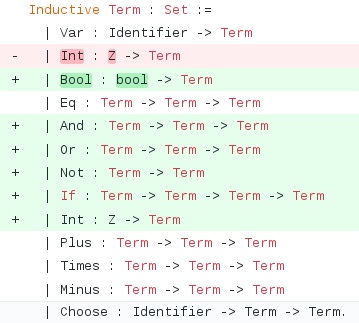
\includegraphics[width=0.7\textwidth]{maintenance/fig/diffs1.png}
\end{minipage}
\hfill
\begin{minipage}{0.57\textwidth}
\centering
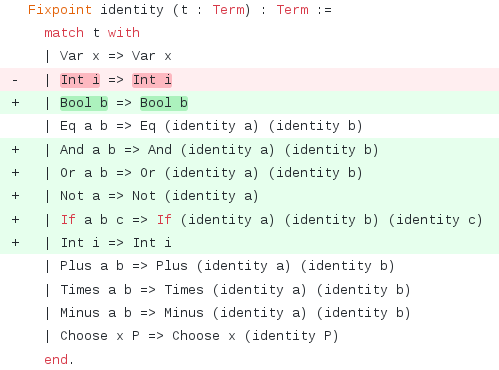
\includegraphics[width=0.7\textwidth]{maintenance/fig/diffs2.png}
\end{minipage}
\caption{A change to an inductive type (left) and corresponding change to a fixpoint (right) that User 5 made in Session 19.}
\label{fig:ex-diff}
\end{figure*}

Classifying changes revealed clusters of related changes.
Further inspection of those clusters revealed common development patterns.
Figure~\ref{tab:userchanges} lists, for each user, the top three changes
by \textbf{Operation} and \textbf{Location} 
(four if there was a tie, and ignoring changes that we found fewer than three times for the user),
the total number of changes that we found,
and the total number of  interactive sessions and self-rated expertise
for reference.
Changes for which more detailed inspection revealed patterns
are highlighted in corresponding colors:
\indpatt{blue} for incremental development,
\refactorpatt{orange} for refactoring, \repairpatt{pink} for
repair, and \pddpatt{grey} for discovery.

The remainder of this section discusses these patterns, complete
with an example, benchmarks, and lessons for automation 
for each.
The benchmarks and lessons for automation are mainly for tool designers:
The benchmarks point to changes in specific sessions, the partial or 
complete automation of which would have helped our users.
The lessons for automation are natural directions for improvements
to proof engineering tools given the patterns we have observed.

The public data repository contains a complete list of the changes
that we classified, as well as a detailed walkthrough of each benchmark.

\subsubsection{Incremental Development of Inductive Types}
\label{sec:pat1}

The most common changes for Users 1 and 5 were adding cases to match statements
(\textbf{Add} \textbf{Cas}) and adding constructors to inductive types
(\textbf{Add} \textbf{Ctr}).
These changes corresponded to incremental development of inductive types,
followed by corresponding extensions to match statements of functions
that destruct over them, or to inductive types that depend
on or relate to them.
This pattern sometimes spanned multiple sessions.
While this pattern was most prevalent for Users 1 and 5, it was also
present for Users 2 and 7.

The diffs in Figure~\ref{fig:ex-diff} show an example change to
an inductive type, along with a corresponding change to a fixpoint.
The change on the left adds five constructors and moves one constructor down.
The change on the right adds five corresponding cases and moves one
corresponding case down.

\paragraph{Benchmark 1}

The example change from \Cref{fig:ex-diff} came from
User 5, Sessions 18, 19, 27, 33, and 35.
There, over the course of three weeks, the user incrementally developed the inductive type \lstinline{Term}
along with a record \lstinline{EpsilonLogic} and fixpoints
\lstinline{simplify} (later renamed to \lstinline{identity}) and \lstinline{free_vars}.

\paragraph{Benchmark 2}

In Sessions 37 and 41, over two days,
User 1 incrementally developed similar inductive types
\lstinline{ST} and \lstinline{GT}, as well as fixpoints
\lstinline{Gamma}, \lstinline{Alpha}, and \lstinline{eq} 
that referred to them.

\paragraph{Lessons for Automation}

Given that several users show this pattern,
this is one use case for which better automation may help.
Automation may help proof engineers adapt other inductive types,
match statements, and proofs after extending inductive types
with new constructors.
We are not aware of any work on adapting related inductive types and 
match statements.
There is some work on adapting proof obligations to new
constructors~\cite{Boite2004},
and a proposed algorithm for generating proofs that satisfy those
obligations~\cite{Mulhern06proofweaving}, but nothing that exists for
a current version of Coq.

\begin{displayquote}
  \textbf{Takeaway}:
  Proof engineers could benefit from automation to help update proofs and definitions
  after adding constructors to inductive types.
  %% Up-to-date automation to help proof engineers adapt definitions
  %% and proofs after extending inductive types is an unaddressed
  %% opportunity make an impact.
\end{displayquote}

\subsubsection{Repetitive Refactoring of Identifiers}
\label{sec:pat2}

Users 1 and 7 showed a pattern of repetitive refactoring, through
qualifying constants after changing imports (\textbf{Qfy} \textbf{Con}),
and renaming identifiers (\textbf{Rnm} \textbf{Idn}) and the constants
that referred to them (\textbf{Rnm} \textbf{Con}), respectively.
This pattern sometimes spanned multiple sessions, and even simple refactorings
sometimes resulted in failures.

Figure~\ref{fig:refactor} shows an example renaming from the five
definitions at the top to the five definitions at the bottom.
The change renames the identifiers of these definitions to
follow the same convention, then makes the corresponding changes
to constants in the bodies of the last two definitions.  

\begin{figure}
  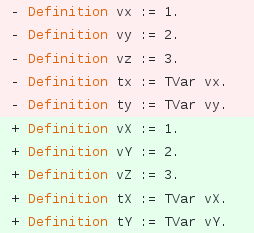
\includegraphics[width=0.19\textwidth]{maintenance/fig/refactor.png}
  \caption{Renaming of definitions in User 7, Session 93.}
  \label{fig:refactor}
\end{figure}

\paragraph{Benchmark 3}

The example from \Cref{fig:refactor} came from User 7, Session 93.
The definition of \lstinline{ty} failed, since User 7 had already
defined an inductive type with that name.
In response, User 7 renamed all of these
to follow the same convention.
This took four attempts, but only a few minutes.

\paragraph{Benchmark 4}

In Session 193, User 7 split the \lstinline{TVar} constructor
of the inductive type \lstinline{ty} into two constructors:
\lstinline{TBVar} and \lstinline{TFVar}. User 7 at the same time
split the fixpoint \lstinline{FV} into \lstinline{FFV} and
\lstinline{FBV}.
In Session 198, User 7 at the same time renamed the broken lemma
\lstinline{b_subst_var_eq} to \lstinline{b_subst_bvar_eq},
and substituted in \lstinline{TBVar} for \lstinline{TVar} in its body.

\paragraph{Benchmark 5}

User 1 imported the \lstinline{List} module in Session 37, commit 10.
After the import, \lstinline{In} referred to the list
membership predicate from the standard library, whereas previously it had
referred to \lstinline{Ensembles.In}. The 6 qualify constant changes that we
found for User 1 were changing \lstinline{In} to \lstinline{Ensembles.In}
inside of three existing definitions.
This took multiple tries per definition,
but only a few minutes in total.

\paragraph{Lessons for Automation}

Refactoring terms (rather than proof scripts) as in
RefactorAgda~\cite{wibergh2019} and Chick~\cite{robert2018}
would have helped our users, but few refactoring tools for
ITPs support this~\cite{PGL-045}, and neither of these are implemented
for Coq.
Supporting making similar changes throughout a program, like Chick does,
may be especially useful.
Semantics-aware refactoring support may take this even further:
A refactoring tool for Coq may, for example, determine that an import
shadows an identifier, compute what the identifier used to refer to,
and refactor appropriately.
Or, it may guide the user to rename terms that refer to other
recently renamed terms.
Both of these would have helped our users.

\begin{displayquote}
  \textbf{Takeaway}:
  Refactoring and renaming tools,
  similar to those available for programmers in languages like Java,
  could also help proof engineers,
  and could potentially be more powerful in ITPs.
%%   Proof refactoring tools should support term refactoring,
%% especially patterns of term refactoring that are informed by Coq's semantics.
\end{displayquote}

\iffalse
Hooking into the REPL, like \toolname does, may help refactoring tools
make these suggestions independently of the UI.
\fi

\subsubsection{Repetitive Repair of Specifications}
\label{sec:pat3}

The top changes that we found for Users 3 and 8 were 
patching arguments (\textbf{Pch} \textbf{Arg}) and replacing functions
(\textbf{Rpl} \textbf{Fun}), respectively.
These corresponded to a pattern of repetitive repair of specifications,
often over several sessions.
Sometimes these repairs were necessary in order for the specification to
type check or for existing tactics to succeed.
Sometimes, after repairing specifications, users also repaired their proofs.

\begin{figure}
  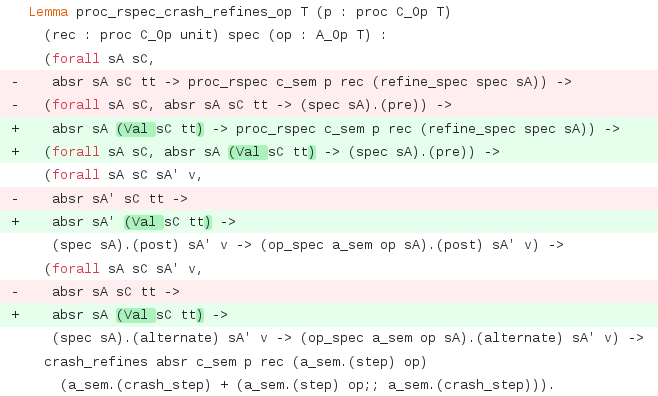
\includegraphics[width=0.47\textwidth]{maintenance/fig/patch.png}
  \caption{Patches to a lemma in User 3, Session 73.}
  \label{fig:patch}
\end{figure}

Figure~\ref{fig:patch} shows an example change patching the arguments
of a lemma. This change wraps two arguments into a single application
in three different hypotheses of a lemma.

\paragraph{Benchmark 6}

11 of the 13 patches to arguments that we found for User 3,
including the example in \Cref{fig:patch}, came from Session 73.
All of these changes similarly wrapped arguments into an application of
\lstinline{Val}.
We suspect that this was due to a change in the definition of \lstinline{absr},
but we were not able to confirm this since
the change in question occurred before the beginning of the study.
The user admitted or aborted the proofs of four of the five
changed lemmas.

\iffalse
For the same reason, we were not able to determine with certainty
that the changes to proofs in that session were corresponding
repairs to match the new specification.
\fi

\paragraph{Benchmark 7}

28 of the 29 replace function changes that we found for User 8
were changes from \lstinline{=} to \lstinline{==} over
the course of about a week in Sessions
2, 14, 37, 40, 65, 79, 108, 125, and 160.
The corresponding proof attempts suggest that while these terms were well-founded with \lstinline{=}, the changes to use \lstinline{==}
may have been necessary to make progress in proofs
using certain tactics.
Sometimes, after making these changes, User 8 also fixed tactics
that had worked before.

\paragraph{Lessons for Automation}

Automation may help with these sorts of repairs to theorems
and proofs. The proof repair tool \textsc{PUMPKIN PATCH} already handles some
repairs to proofs after changes to both
\textbf{Content}~\cite{Ringer2018} and \textbf{Structure}~\cite{Ringer2019}, but has support for repairing the theorem statement itself only in
the latter case, and only for a specific class of changes to inductive types.
These changes provide examples where changing the theorem type is also
desirable, and may make good benchmarks for further development
to support this.

\begin{displayquote}
  \textbf{Takeaway}:
  Proof repair tools should repair programs and specifications,
  not just proofs.
\end{displayquote}

\subsubsection{Interactive Discovery of Programs and Specifications}
\label{sec:pat4}

In Q1 (Section~\ref{sec:q1}), we found that users most often fixed
proofs by stepping up outside of proofs and changing other things.
Our observations from Q2 are consistent with this,
and give some insight into the details.
Changes from Users 3, 7, 8, and 10 all revealed a pattern of interactive
discovery of programs and specifications:
In some cases, these users discovered bugs in their programs during a
proof attempt or test.
In other cases, these users discovered that their specifications were
incorrect, too weak, or difficult to work with.
Users sometimes assigned temporary names to lemmas or theorems,
then renamed them only after finalizing their types.
Even experts made mistakes in programs and theorem statements
(perhaps they were the ones catching them most effectively).

\begin{figure}
  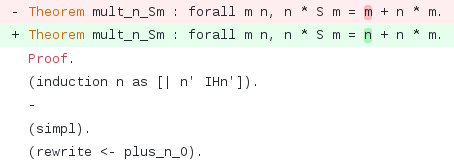
\includegraphics[width=0.35\textwidth]{maintenance/fig/bad.png}
  \caption{A partial attempt at proving and later correction to an incorrect theorem from User 3, Session 11377 (tactic formatting is not preserved in the data
that \toolname receives).}
  \label{fig:bad}
\end{figure}

Figure~\ref{fig:bad} shows an example of catching a bug in a specification
during an attempted proof attempt. The theorem
before the change is impossible (let \lstinline{m} be \lstinline{3} 
and \lstinline{n} be \lstinline{1}).
After attempting to prove it and reaching this goal:

\begin{lstlisting}
  m : nat
  --------
  0 = m
\end{lstlisting}
the user steps up and fixes the theorem statement by replacing an argument
(\textbf{Rpl} \textbf{Arg}), then later finishes the proof.

\paragraph{Benchmark 8}

The change from \Cref{fig:bad} can be found in User 3, Session 11377.
The same session contains changes to the same theorem by
moving arguments (\textbf{Mov} \textbf{Arg}).
The user succeeded at the proof after about three minutes.
%All of the changes moving arguments that we found for User 3
%corresponded to interactive discovery of fixpoints and theorems.

\paragraph{Benchmark 9}

In Session 13, commit 11, User 10 patched a case (\textbf{Pch} \textbf{Cas})
of a fixpoint \lstinline{fib'} after testing.
This took the user about thirty seconds.
The fixpoint \lstinline{fib'} itself may have been used to 
test a different function.

\paragraph{Benchmark 10}

User 7 mainly demonstrated this pattern through
adding and moving hypotheses (\textbf{Add} and \textbf{Mov} \textbf{Hyp}).
The latter most often
corresponded to generalizing the inductive hypothesis 
after a partial proof attempt by swapping theorem hypotheses,
in some cases in order to induct over a different hypothesis 
altogether.
We found such changes in Sessions 19, 56, 93, 94, 104, 110,
153, 159, and 176.
See, for example, \lstinline{match_ty__value_type_l} in Session 94,
commit 15.

\paragraph{Benchmark 11}

In Session 2, User 7 temporarily named a lemma
\lstinline{weird_trans}, then renamed it to \lstinline{sub_r_nf__trans}
by Session 10 after finalizing its type after several partial
proof attempts over the course of about a day and a half.

\paragraph{Lessons for Automation}

The effect of discovering bugs by attempting a proof accounts for some
of the benefits of verification~\cite{murraybp}.
It makes sense, then, to continue to build automation to support users
in finding and fixing those bugs.
One possible unexplored avenue for this is integrating repair tools
with QuickChick~\cite{Paraskevopoulou2015} for testing specifications,
or with the \lstinline{induct} tactic from FRAP~\cite{FRAPBook}
or the hypothesis renaming functionality from CoqPIE~\cite{Roe2016}
for simple generalization of inductive hypotheses.
Integrating tools for discovering lemma and theorem names~\cite{Aspinall2016b}
during the development process may help users who use temporary names.
Above all, repair is not just something that happens to stable proof
developments---change is everywhere in developing those programs and
proofs to begin with.

\begin{displayquote}
  \textbf{Takeaway}: Integrating tools for proof repair with tools
  for discovery and development of specifications
  is an unaddressed opportunity to support proof engineers.
\end{displayquote}


%\section{Conclusions \& Future Work}
\label{sec:discussion}

We built \toolname, a Coq plugin that remotely collects fine-grained
proof development data in a way that is decoupled from the UI.
Using \toolname, we collected data on changes to proofs, programs,
and specifications at a level of granularity not previously
seen for an ITP.
Visualization and analysis of this data revealed evidence in our study
population of development patterns, at times confirming folk knowledge---like 
that discovering  the correct program or specification was often a
conversation with the proof itself, even for experts---and providing
useful insights and benchmarks for tools.

The infrastructure that we have built and the data that we have collected
using it are publicly available.
We hope to see it used as benchmarks for the improvement of
proof engineering tools, and as data for future studies.
We hope to see the infrastructure that we have built reused or
adapted to other ITPs for future studies.

\paragraph{Three Wishes}
We would like for our experiences building and using \toolname
to help the community conduct more studies of proof development processes.
We thus conclude with three wishes, the fulfillment of which would help
address the challenges that we encountered along the way:

\begin{enumerate}
\item Better abstraction of user environments (Section~\ref{sec:wish1})
\item More information about user interaction (Section~\ref{sec:wish2})
\item More users (Section~\ref{sec:wish3})
\end{enumerate}
We discuss how to grant each wish both at the level of study design
and at the level of ITP design in order to facilitate future studies of 
this kind.

\subsection{Wish: Better Abstraction of User Environments}
\label{sec:wish1}

In order to cast as broad of a net as possible for potential users, we
designed \toolname to be independent of the UI, 
the version of Coq, and the build system. Coq's plugin infrastructure
and interaction model offered a promising avenue for this,
%Together with the Coq developers, we were able to extend the plugin API
%with a hook to listen to Coq's REPL.
and Coq's resource file infrastructure meant that users could load the plugin
universally with just one LOC in one location.
All of this gave us the impression of independence from the details of
the UI, ITP version, and build system.

We later found that, while this infrastructure was useful,
the impression of total independence was somewhat of an illusion; 
all of these details mattered.
In particular, while \toolname itself was UI-independent, the analyses
that we ran did not achieve full independence.
For example, we found that depending on the version of Coq and what
event triggers a cancellation, different UIs use different mechanisms
for cancellation (recall these mechanisms from Section~\ref{sec:plugin}). 
Our analyses had to deal with all of these mechanisms.

In addition, partway through the study, we received a bug 
report that noted that one common build system for Coq compiles files by
default using a flag that disables loading the Coq resource file.
This is one possible explanation for the lack of data that some users sent.
To remedy this, we must ask future users of \toolname
to compile all of their Coq projects without using this flag;
we have updated the \toolname documentation to account for this. 

\paragraph{The Study Designer} Without help from the ITP designer,
the study designer cannot achieve full abstraction from these details.
The study designer may, however, work around the lack of full abstraction.
We recommend testing the study infrastructure with 
many different environments for many different scenarios.
It may help to identify potential users early and survey their
development environments before even beginning to test,
covering likely scenarios in advance.
It may also help to build in a short trial period on the final users
before the final data collection begins, thereby
covering their particular development environments.
The latter has the additional benefit of giving the study designer
time to discover and discuss with users possible confounding
variables for analysis, like development style or project phase.

We had the foresight to test \toolname with \lstinline{coqtop}, 
Proof General, and CoqIDE, but we did not anticipate User 5's custom
UI, which treated failures differently from the others.
We also did not anticipate the behavior of different
build systems on Coq's resource file, since we tested only one
build configuration.
We could have avoided both of these issues with our recommendations.
Instead, we had to work around both issues after deployment.

\paragraph{The ITP Designer} 
Most of the power to grant this wish is in the hands of the ITP designer.
Full abstraction over development environments may not be possible, but the
ITP designer may design the interaction model with this as a goal.
The REPL and state machine already strive for this---and come
close to achieving it---but their current implementations in Coq fall short.
Improvements to abstraction here may be minimal, like
providing fewer mechanisms for UIs to accomplish the same thing,
or providing a way to guarantee that a plugin is always loaded for all
build systems.

For a more radical approach, the ITP designer may look to other 
interaction models.
For example, Isabelle/HOL has recently moved away from its REPL,
instead favoring the Prover IDE (PIDE)~\cite{Wenzel2012} framework
as its interaction model.
With PIDE, UIs and ITPs communicate using an asynchronous protocol to manage
versions of a document~\cite{Wenzel2014}, annotating the document with 
new information when it becomes available~\cite{Wenzel2012}.
Personal communication suggests that there is an ongoing attempt to 
to centralize functionality like the build system into PIDE.
While centralization may limit the potential for customization by different
UIs, it may make studies of fine-grained proof development data easier,
since the instrumentation may occur at a higher level,
guaranteeing more uniform interaction.

\subsection{Wish: More Information about User Interaction}
\label{sec:wish2}

By observing state machine messages through the plugin API,
we were able to log data at high enough granularity to reconstruct
hundreds of interactive sessions. This helped us identify incremental
changes to tactics and terms that are difficult to gather from other sources.

The hooks that we designed together with the Coq developers, however, 
were not perfect.
There was no way for us to use those hooks to listen to the messages
that Coq sent back to the UI.
Making this change would have required modifying Coq again, and by the time
we realized this, it was too late.
Listening to those responses would have given us more insight into user
behavior.
It would have also helped us distinguish between failures and stepping up.
Instead, we had to distinguish between these using IDE-specific heuristics,
which left us with no automatic way to distinguish failures from stepping up
for User 5's custom UI.

We also found that once we had collected granular data, 
analyzing it was sometimes difficult. 
For example, sometimes users defined a term, stepped up and changed
an earlier term, then stepped back down and changed the original term.
For such a change, our visualization script constructed 3 consecutive commits;
to determine that the original term had changed, we had to look at 
the difference between the 1st and the 3rd commits.
Sometimes, changes occurred over tens of commits, or over several sessions.
Thus, manual analysis of changes for Q2 was tedious, and involved
not only inspecting thousands of diffs but also understanding each 
session well enough to track term information over time.

We considered automating the analysis for Q2, but we found
automatically classifying changes in terms to be prohibitively difficult.
While part of this was due to the inherent difficulty of the problem,
part of this was also due to missing information:
When the UI backed up to an earlier state, we did not know what was below 
the command or tactic corresponding to that state in the file. 
So, when a user copied and pasted a term and then modified both versions,
or made several changes at once to a term before stepping 
down below it, even manually deciding whether it was the same term 
that had changed or a new term entirely proved to be difficult.

\paragraph{The Study Designer}
To grant this wish, we recommend that the study designer run a beta test, complete with analysis, as we did---and that they do so early,
as we did not.
That way, there is enough time to address needs discovered during testing,
for example by communicating with ITP designers.
It may also help to use multiple methods for data collection,
for example by augmenting the collected data with information from the IDE
to track the state of definitions in the file below the location to
which the user has stepped.

The beta testing phase was extremely useful to us; as a result we
reworked our server infrastructure to receive and easily
analyze larger amounts of data, and we tested data backup
infrastructure and network failure resilience code. 
We also discovered and reported a 
bug\footnote{\url{http://github.com/coq/coq/issues/8989}} in CoqIDE and 
Proof General that had made it impossible for us to tell which 
sessions corresponded to which files; the fix was marked as critical 
and backported to Coq 8.9, so only the analyses for Users 5 (custom UI), 8 (Coq 8.8), and 10 (Coq 8.8) were impacted.
However, while we discovered the lack of response information in the plugin hooks
during this period, we did not have enough time to coordinate with Coq developers on
changes to the hooks. 
Leaving more time between testing and the final study would have helped us.

\paragraph{The ITP Designer} 
By implementing hooks like the one that we helped implement for Coq,
the ITP designer can make it easier for researchers to study 
proof development processes. 
To grant this wish, we recommend that these hooks expose not just 
request information, but also response information, 
especially error information.

Augmenting the interaction model with more information
about the file may also help.
For example,
the interaction model could expose a simple and uniform way for UIs
to track that a definition in a new state corresponds to a definition 
in a previous state (that is, that the user did not remove that
definition from the file and replace it with something entirely new). 
This could make it much simpler for an analysis to track changes to a definition over time,
and to choose the granularity with which to inspect changes.
There is some tension between this and the wish for abstraction from
Section~\ref{sec:wish1}, but it may be worth weighing the tradeoffs.

\subsection{Wish: More Users}
\label{sec:wish3}

We attempted to recruit a large and representative sample of Coq proof
engineers.
In our attempts to recruit users, we contacted programming
languages groups at several universities that were known to be working
with Coq, and emailed \lstinline{coq-club} with our project
pitch. We included a promotional video in the hopes of
attracting as many users as possible.

In the end, however, we were able to recruit only 12 users,
all of whom were intermediate through expert users with at least two years
of Coq experience. We received interactive sessions for just 8 of 12
of these users. While this data was rich and granular, with just 8 users,
we were not able to reach broad conclusions about proof engineers more generally.

Part of this was likely due to the demographics of the
community: Compared to other programming environments,
Coq has only a small number of users,
many of whom have or are pursuing graduate degrees.
However, part of this may have been due to
deterrents in our screening process, or poor incentives for our users.

\paragraph{The Study Designer}
The study designer may fulfill this in part by casting as broad of a net
as possible, carefully considering any deterrents in screening criteria.
It may help to use welcoming language to encourage potential users
who are unsure if they qualify.
To reach beginner users, it may help to recruit students.
To reach a more international audience, it may help to distribute
promotional materials and consent forms in multiple languages.
It may also help to consider incentives that appeal to proof engineers.
However, until the ITP user community grows significantly, it will continue 
to be difficult to conduct large-scale studies of proof engineering.

We reached users from different institutions, but
most of our users had similar levels of expertise. We suspect that this was
in part because we asked for users to have at least a year of 
experience using Coq, so as to avoid mixing in data from
users learning Coq for the first time.
We also required fluency in English to ensure that users understood
the consent forms.
Both of these may have deterred users.
One potential user who did not participate noted that we did not make
it clear in our recruitment materials that data from occasional rather
than frequent Coq users was still useful to us.
The same potential user noted that we could have engaged more
with community leaders, thereby giving others in the community
more incentive to participate.
We considered monetary incentives, but ultimately decided they were less
tempting to the community than appeals to improving tools.
Perhaps this was misguided or attracted a more advanced population,
and perhaps we could have considered a different incentive.

\paragraph{The ITP Designer}
The ITP designer may help reduce the costs of participating in these studies. 
We suspect that the primary gains here will come from continuing to 
break down barriers to using plugins and other outside tooling. 
Some examples of this include reducing the brittleness of plugin APIs 
over time, improving build and distribution systems, making it possible 
to prove that a plugin does not interact with a kernel in a way that 
could compromise soundness of the system, 
and providing more support for users who port proof developments
and tools between ITP versions.

Of course, continuing to improve the ITP itself may continue 
to expand the community to reach more users. 
This may cause a positive feedback loop, helping to collect more data 
in order to drive further improvements to the ITP, in turn continuing to help
the community grow.




%\chapter{Related Work}

% TODO whatever else isn't here yet, and some of this might be factored out or partially factored out---all papers, including survey, plus generals

\section{Programs}

\subsection*{Program Refactoring} 

Refactoring~\cite{Mens:2004:SSR:972215.972286}.

\subsection*{Program Repair} 

% From PUMPKIN PATCH, unchanged

Adapting proofs to changes is essentially program repair
for dependently typed languages. 
Program repair tools for 
languages with non-dependent type 
systems~\cite{Pei:2014:APR:2731750.2731779, Long:2016:APG:2837614.2837617, Le:2017:SSS:3106237.3106309, Mechtaev:2016:ASM:2884781.2884807, Monperrus2015} 
may have applications in the context of a dependently typed language.
Similarly, our work may have applications within program repair in these languages:
Future applications of our approach may repurpose it to repair programs for functional languages.

\subsection*{Ornaments}

% From PUMPKIN PATCH, unchanged

Ornaments~\cite{Dagand17jfp, Williams:2014:OP:2633628.2633631}
separate the computational and logical components of a datatype, and may
make proofs more resilient to datatype changes.

\subsection*{Programming by Example}

% From PUMPKIN PATCH, unchanged

Our approach generalizes an example that the programmer provides.
This is similar to programming by example, a subfield of 
program synthesis~\cite{DBLP:journals/ftpl/GulwaniPS17}. 
This field addresses different challenges in different logics,
but may drive solutions to similar problems in a dependently typed language.

\subsection*{Differencing \& Incremental Computation}

% From PUMPKIN PATCH, unchanged

Existing work in differencing and incremental computation may help 
improve our semantic differencing component.
Type-directed diffing~\cite{Miraldo:2017:TDS:3122975.3122976}
finds differences in algebraic data types.
Semantics-based change impact analysis~\cite{Autexier:2010:SCI:1860559.1860580} models semantic differences
between documents.
Differential assertion checking~\cite{differential-assertion-checking-2} analyzes different
versions of a program for relative correctness with respect to a specification.
Incremental $\lambda$-calculus~\cite{Cai:2014:TCH:2594291.2594304} introduces a general model for program changes.
All of these may be useful for improving semantic differencing.

\section{Proofs}

\subsection*{Proof Reuse}

% From PUMPKIN PATCH, unchanged

Our approach reimagines the problem of proof reuse in the context of proof automation.
While we focus on changes that occur over time, traditional proof reuse techniques can help
improve our approach.
Existing work in proof reuse focuses on transferring proofs between isomorphisms,
either through extending the type system~\cite{Barthe:2001:TIP:646793.704711} or through an automatic method~\cite{Magaud2002}.
This is later generalized and implemented in Isabelle~\cite{Huffman2013} and Coq~\cite{ZimmermannH15, tabareau:hal-01559073};
later methods can also handle implications. 
%Transfer tactics apply these functions but do not infer them, while our approach
%infers these functions but does not apply them.
Integrating a transfer tactic with a proof patch finding tool will create an end-to-end
tool that can both find patches and apply them automatically.

Proof reuse for extended inductive types~\cite{Boite2004} adapts proof obligations
to structural changes in inductive types. Later work~\cite{Mulhern06proofweaving} proposes a method
to generate proofs for new constructors. These approaches may be useful when extending the differencing
component to handle structural changes. Existing work in theorem reuse and proof generalization~\cite{Felty1994, pons00, Johnsen2004} abstracts existing proofs for reusability, and may be useful
for improving the abstraction component.
Our work focuses on the components critical to searching for patches; these complementary approaches
can drive improvements to the components.

\subsection*{Proof Evolution}

% From PUMPKIN PATCH, unchanged

There is a small body of work on change and dependency management for verification,
both to evaluate impact of potential changes and maximize reuse~\cite{873647, Autexier:2010:CMH:1986659.1986663}
and to optimize build performance~\cite{Celik:2017:IRP:3155562.3155588}.
These approaches may help isolate changes, which is necessary to identify future benchmarks, integrate
with CI systems, and fully support version updates.

\subsection*{Proof Refactoring}

\subsection*{Proof Repair}

\subsection*{Proof Design}

% From PUMPKIN PATCH, unchanged:

Existing proof engineering work addresses brittleness
by planning for changes~\cite{proof-eng} and designing theorems and proofs that make maintenance less of an issue.
Design principles for specific domains (such as formal metatheory~\cite{Aydemir2008, Delaware2013POPL, Delaware2013ICFP})
can make verification more tractable. CertiKOS~\cite{certikos} introduces the idea of a deep specification to
ease verification of large systems.
These design principles and frameworks are complementary to our approach.
Even when programmers use informed design principles,
changes outside of the programmer's control can break proofs;
our approach addresses these changes.

\subsection*{Proof Automation}

% From PUMPKIN PATCH, unchanged:

We address a missed opportunity in proof automation for ITP: searching
for patches that can fix broken proofs.
This is complementary to existing automation techniques. Nonetheless, there is a wealth
of work in proof automation that makes proofs more resilient to change.
Powerful tactics like \lstinline{crush}~\cite{chlipala:cpdt} can make
proofs more resilient to changes. 
Hammers like Isabelle's sledgehammer~\cite{Blanchette2013} can make proofs agnostic to some low-level changes.
Recent work~\cite{coqhammer} paves the way for a hammer in Coq.
Even the most powerful tactics cannot address all changes;
our hope is to open more possibilities for automation.

Powerful project-specific tactics~\cite{chlipala:cpdt, Chlipala2013} can help prevent low-level maintenance tasks.
Writing these tactics requires good engineering~\cite{Gonthier2011} and domain-specific knowledge,
and these tactics still sometimes break in the face of change.
A future patching tool may be able to repair tactics; the debugging process
for adapting a tactic is not too dissimilar to providing an example to a tool.

Rippling~\cite{rippling} is a technique for automating inductive proofs that uses restricted rewrite rules to
guide the inductive hypothesis toward the conclusion; this may guide improvements to the
differencing, abstraction, and specialization components.
The abstraction and factoring components address specific classes of unification problems;
recent developments to higher-order unification~\cite{Miller:2012:PHL:2331097} may help
improve these components.
Lean~\cite{selsam:lean} introduces the first congruence closure algorithm for dependent type theory that
relies only on the Uniqueness of Identity Proofs (UIP) axiom. While UIP is not fundamental to Coq,
it is frequently assumed as an axiom; when it is, it may be tractable to use a similar algorithm to improve the tool.

GALILEO~\cite{bundyreasoning} repairs faulty physics theories
in the context of a classical higher-order logic (HOL); there is preliminary work extending this
style of repair to mathematical proofs. 
Knowledge-sharing methods~\cite{tgck-cicm14} can adapt some proofs across different representations of HOL.
These complementary approaches may guide extensions to support decidable domains and classical logics.

\subsection*{Transport}

\subsection*{Parametricity}

\subsection*{Refinement}




\iffalse
(This subsection is not done yet, but not really needed to understand flow of paper.)

There are a lot of development processes people use to make proofs less likely to break to begin with (survey paper).

Two examples I like: First, affinity lemmas and reference to \lstinline{zip} example.
Second, better tactics like from CPDT and how could help is in \lstinline{zip} example.

Quick summary of some other ideas from survey paper.
For more, see the survey paper.

In that case, it may help us to define a more general \lstinline{patch} corresponding to the change:

\begin{lstlisting}
Lemma patch:
  forall {T$_1$} {T$_2$} (l$_1$ : list T$_1$) (l$_2$ : list T$_2$) (P : list (T$_1$ * T$_2$) $\rightarrow$ Type),
    length l$_1$ = length l$_2$ $\rightarrow$ 
    P (zip_same_length l$_1$ l$_2$) $\rightarrow$ 
    P (zip l$_1$ l$_2$).
Proof.
  intros. unfold zip.
  induction (eq_dec (length l$_1$) (length l$_2$)); simpl; auto.
  apply False_rect. auto.
Defined.
\end{lstlisting}
This says that it is possible to get between \textit{any} proof about \lstinline{zip_same_length}
and \textit{any} proof about \lstinline{zip}.
We can apply this in proofs about \lstinline{zip}:

\begin{lstlisting}
Proof.
  (@\codediff{intros. apply patch; auto.}@)
  (@\codediff{revert H. revert l$_2$.}@)
  induction l$_1$ as [|t$_1$ tl$_1$ IHtl$_1$].
  - auto.
  - intros l$_2$. induction l$_2$ as [|t$_2$ tl$_2$ IHtl$_2$].
    + intros H. auto.
    + intros H. simpl. rewrite IHtl1; auto.
Defined.
\end{lstlisting}
In Section~\ref{TODO}, I will show how \sysname can automatically extract patches like \lstinline{patch} % TODO would be great if it worked for this example
from example changes in proofs.
\fi

